\documentclass{article}

\usepackage[italian]{babel}
\usepackage[letterpaper,top=2cm,bottom=2cm,left=3cm,right=3cm,marginparwidth=1.75cm]{geometry}
\usepackage{amsmath}
\usepackage{graphicx}
\usepackage{subcaption}
\usepackage{textcomp}
\usepackage{ragged2e}
\usepackage[dvipsnames]{xcolor}
\usepackage{fancyhdr}
\usepackage[colorlinks=true, allcolors=blue,
            pdfauthor={Matteo Drago},
            pdftitle={Bivacco Malga Lavacchio},
            pdfsubject={Diario bivacchi e trekking},
            pdfkeywords={bivacco, montagna, trekking, diario}]{hyperref}
                
\title{\textbf{Bivacco Malga Lavacchio - 1369 m s.l.m}}
\author{Matteo Drago}

% ==========================================================
% Impostazioni per il logo in ogni pagina
% ==========================================================
\pagestyle{fancy}
\fancyhf{} % Pulisce tutti i campi di intestazione e piè di pagina
\fancyhead[R]{
\includegraphics[height=1.5cm]{images/toothless.jpeg}} % Posiziona il logo a destra (R) nell'intestazione
\renewcommand{\headrulewidth}{0pt} % Rimuove la linea orizzontale nell'intestazione (opzionale)


\begin{document}
\maketitle
\thispagestyle{fancy} % Aggiungi questa riga

\begin{abstract}
Questo documento raccoglie e organizza le informazioni che ho acquisito nel corso degli anni sui bivacchi, basate sulle mie esperienze dirette. Sebbene non si proponga come una guida esaustiva e perfetta, offre il minimo indispensabile per una buona vita in bivacco, con consigli pratici e diretti per chiunque desideri affrontare al meglio queste pazze ma piacevoli avventure.
\end{abstract}

\section{Il bivacco}

% ==========================================================
% Immagine a sinistra, testo a destra allineato in alto
% ==========================================================
\noindent
\begin{minipage}[t]{0.45\textwidth}
  \vspace{0pt} % forza l'allineamento in alto
  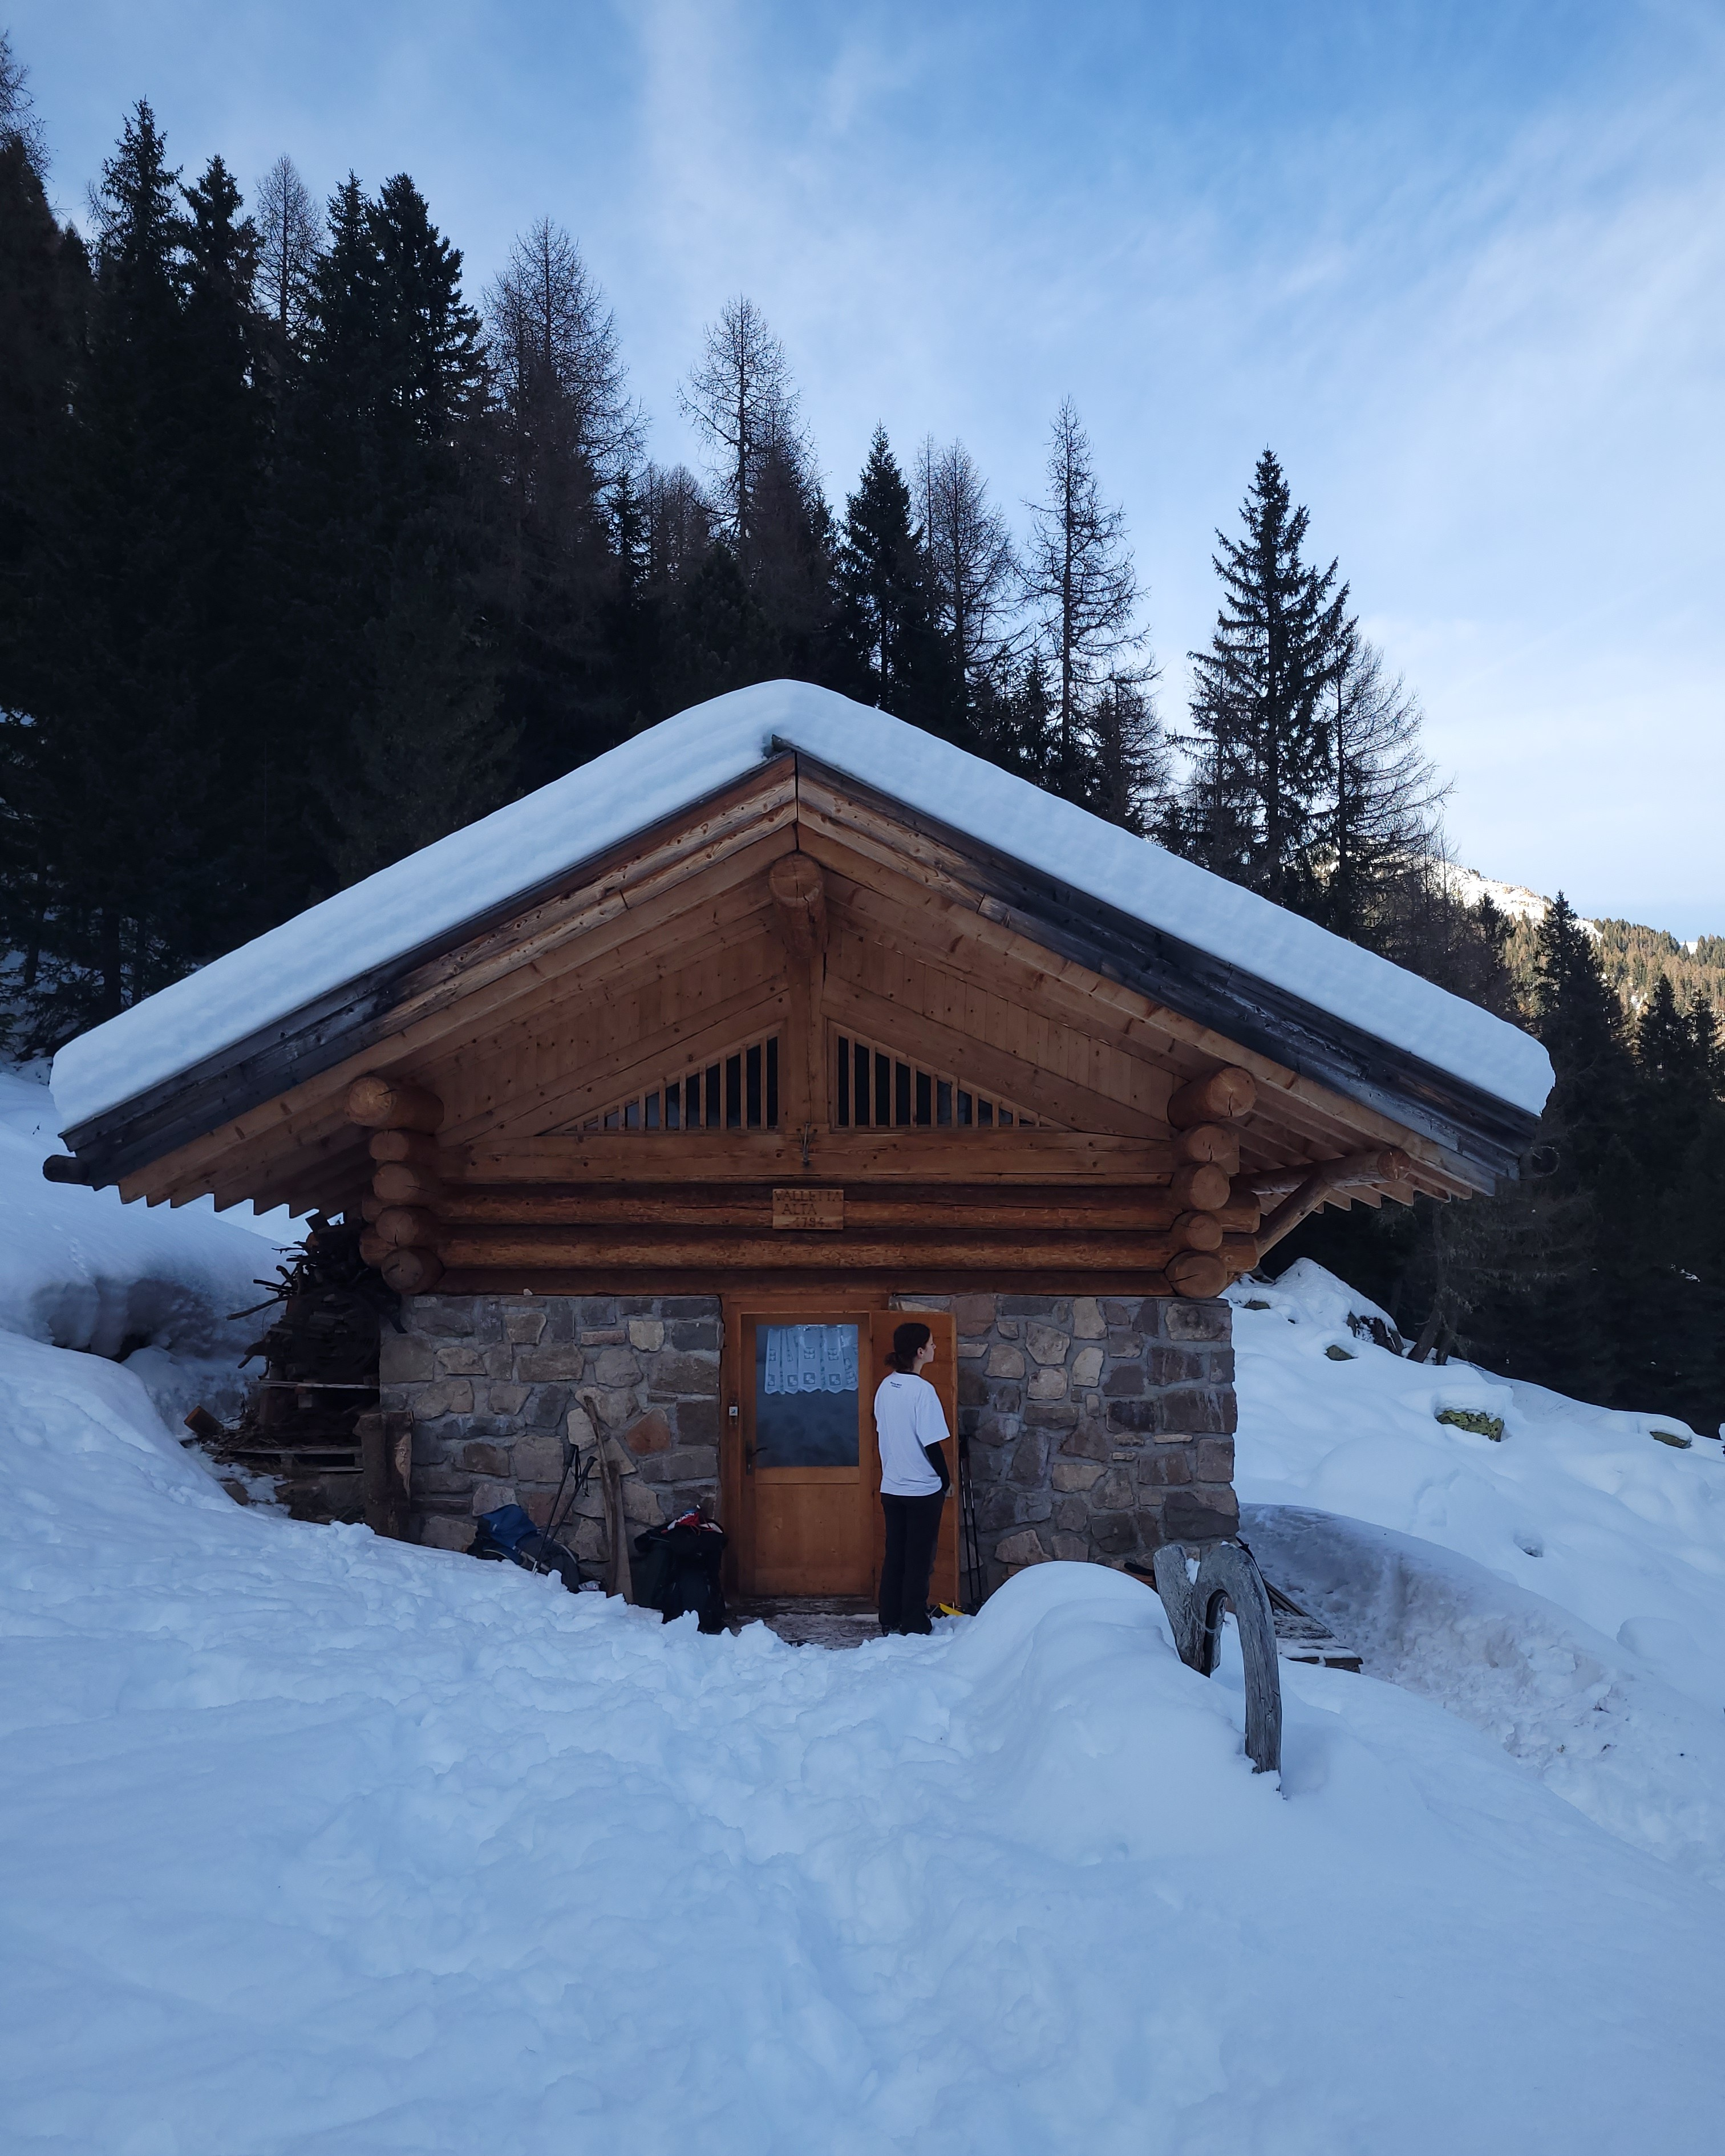
\includegraphics[width=\linewidth]{images/bivacco.jpg}
\end{minipage}%
\hfill
\begin{minipage}[t]{0.5\textwidth}
  \vspace{0pt} % forza l'allineamento in alto
  
  Gruppo montuoso\\
  \textbf{\large Monte Baldo}
  \\[1em] % Aggiunge una riga vuota qui
  Località\\
  \textbf{\large Piani di Lavacchio}
  \\[1em] % Aggiunge una riga vuota qui
  Comune\\  
  \textbf{\large Avio}
  \\[1em] % Aggiunge una riga vuota qui
  Altezza\\  
  \textbf{\large 1369 m s.l.m.}
  \\[1em] % Aggiunge una riga vuota qui
  Apertura\\  
  \textbf{\large Non gestito, sempre aperto}

\end{minipage}

\subsection{Caratteristiche}
Il Bivacco Malga Lavacchio è un'ex "casera", proprietà del Comune di Avio e affidata alla Sezione di Avio della SAT.

È circondato da un recinto (utile dato che nella zona sono stati avvistati dei lupi) ed è strutturato su due piani.
\begin{itemize}
    \item \textbf{Piano terra}: due tavoli con panche, un camino e una dispensa con vario materiale (caffè, bombole di riserva, risotti, ecc.).
    \item \textbf{Piano superiore}: diversi materassi che permettono a circa 6-7 persone di dormire comode (sfruttando anche il piano terra si può arrivare facilmente a 15+).
    \item \textbf{Posti letto extra}: una zona chiusa a chiave di proprietà del SAT (risultata scassinata) offre un'altra decina di posti però non è lasciata in buone condizioni.
\end{itemize}

L'esperienza al bivacco è ottima sia in estate che in inverno, poiché il camino permette di riscaldare molto bene l'ambiente, specialmente quello superiore. \textbf{\textcolor{OrangeRed}{Invito, tuttavia, a prestare molta attenzione al camino: il fumo fatica molto a uscire dalla canna fumaria, dato che il passaggio dell'aria è stato bloccato sul muro retrostante (noi ci siamo svegliati nel mezzo della notte con tutto il bivacco affumicato, rischiando di soffocare).}}

Nelle zone limitrofe al bivacco sono assenti fonti d'acqua; tuttavia, ricavare la legna è molto semplice data la presenza di un vasto bosco che lo circonda.

\section{Come ci siamo arrivati}
Abbiamo parcheggiato la macchina a Ferrara di Monte Baldo e da li ci siamo incamminati. Pausa pranzo lungo il sentiero per poi arrivare verso le 16.00 alla malga. Il giorno dopo abbiamo proseguito il nostro giro ad anello per poi tornare alla macchina.


\begin{figure}[htbp!]
    \centering
    % Colonna di sinistra, allineata in alto
    \begin{subfigure}[t]{0.45\textwidth}
        \centering
        \vspace{0pt} % Forziamo l'allineamento in alto
        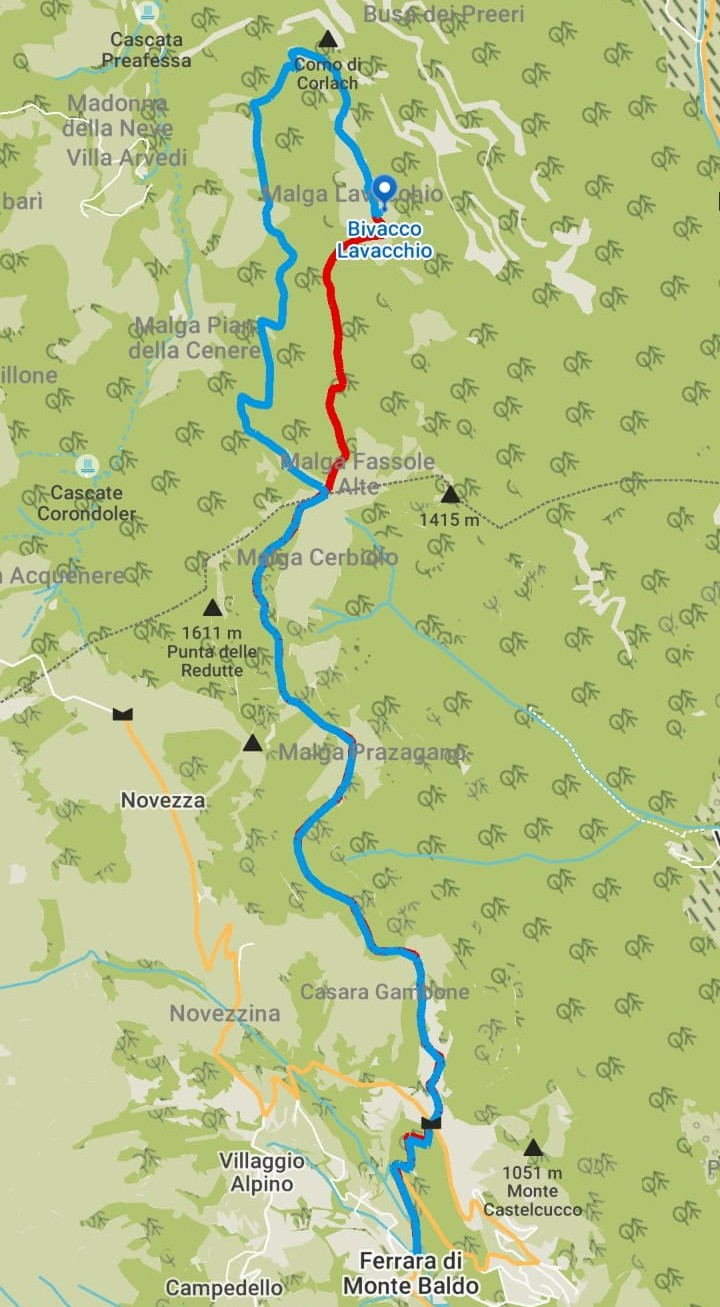
\includegraphics[width=\textwidth]{images/sentiero_mapsMe.jpg}
        \caption{Sentiero su Maps.Me.}
        \label{fig:foto_lunga}
    \end{subfigure}
    \hfill
    % Colonna di destra, allineata in alto
    \begin{subfigure}[t]{0.45\textwidth}
        \centering
        \vspace{0pt} % Forziamo l'allineamento in alto anche qui
        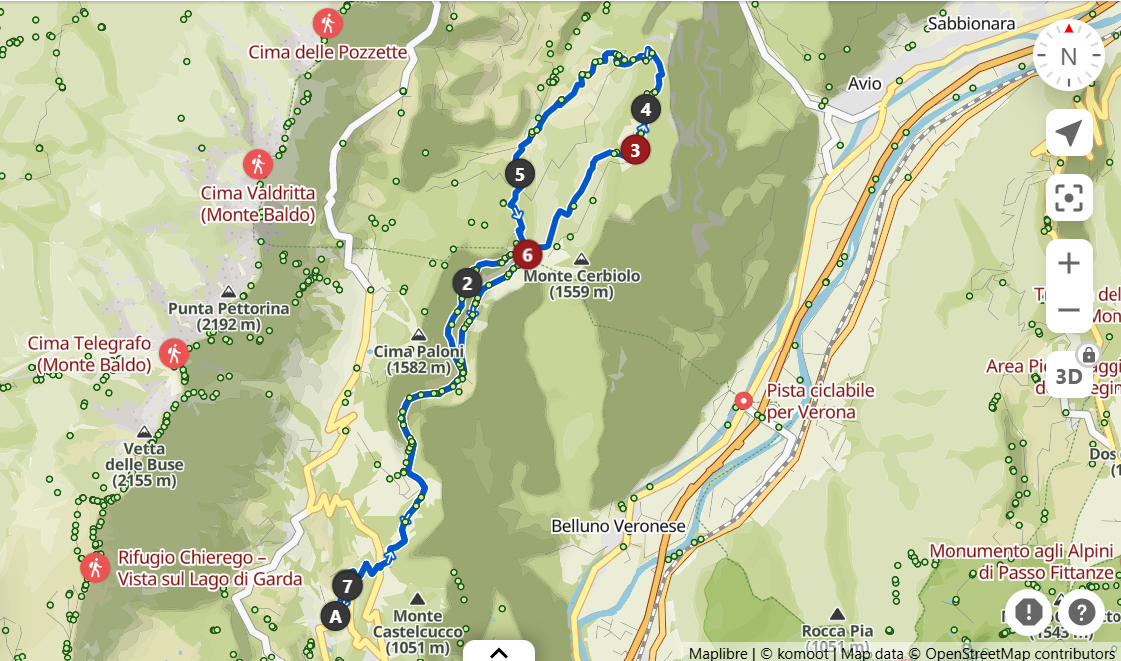
\includegraphics[width=\textwidth]{images/sentiero_komoot.png}
        \caption{Sentiero su Komoot.}
        \label{fig:foto_corta1}
        \vspace{1em} % Aggiunge un po' di spazio tra le due foto
        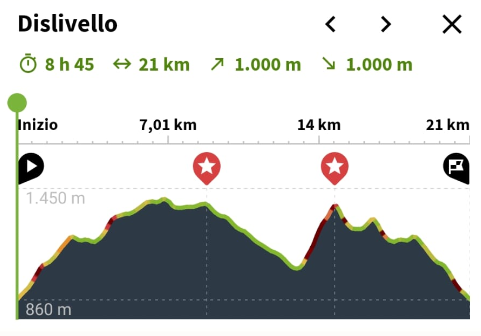
\includegraphics[width=\textwidth]{images/profilo_altimetrico.png}
        \caption{Profilo altimetrico del percorso.}
        \label{fig:foto_corta2}
    \end{subfigure}
    % Didascalia generale per l'intera figura
    \caption{Il sentiero e i dettagli del percorso.}
    \label{fig:panoramica_dettagli}
\end{figure}


\section{Non ti scordar di me}
\textbf{\textcolor{BurntOrange}{Ricorda: il bivacco è un bene comune. Il suo futuro dipende dal rispetto e dal senso civico dei visitatori. Usalo con cura e lascialo più pulito di come l'hai trovato.}}


\section{Esperienza personale}
Questa è stata la nostra prima esperienza in bivacco da soli, siamo arrivati a Ferrara di Monte Baldo verso le 10.00 e il cammino per arrivarci è stato molto piacevole, con un paesaggio molto suggestivo e incontri inaspettati (professore di musica delle medie). Quando siamo arrivati al bivacco c'erano già 3 ragazzi che abbiamo successivamente scoperto essere li già da qualche giorno. Come già detto la nottata è stata caratterizzata da un problemino con il camino, ma oltre a quello è andato tutto liscio. 


\section{Alcune foto}

\begin{figure}[htbp!]
    \centering
    % Prima immagine
    \begin{subfigure}[b]{0.45\textwidth}
        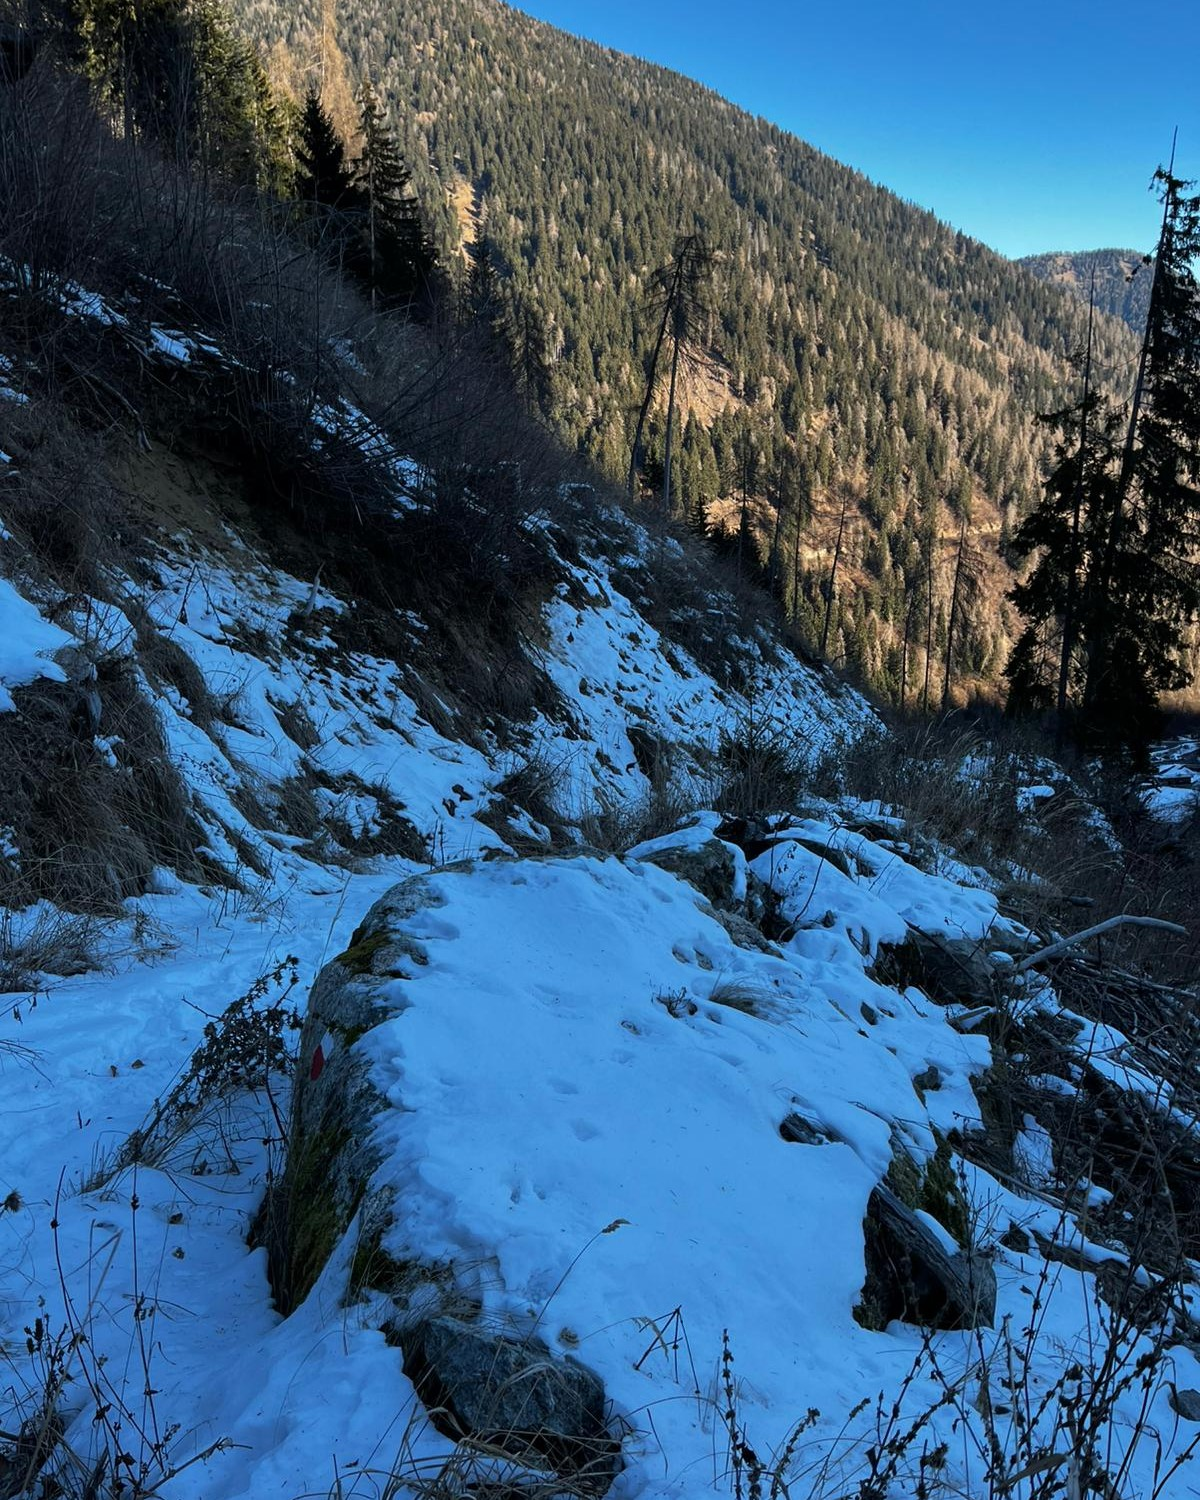
\includegraphics[width=\textwidth]{images/foto_sentiero.jpg}
        \caption{Sentiero.}
        \label{fig:prima_foto}
    \end{subfigure}
    \hfill
    % Seconda immagine
    \begin{subfigure}[b]{0.45\textwidth}
        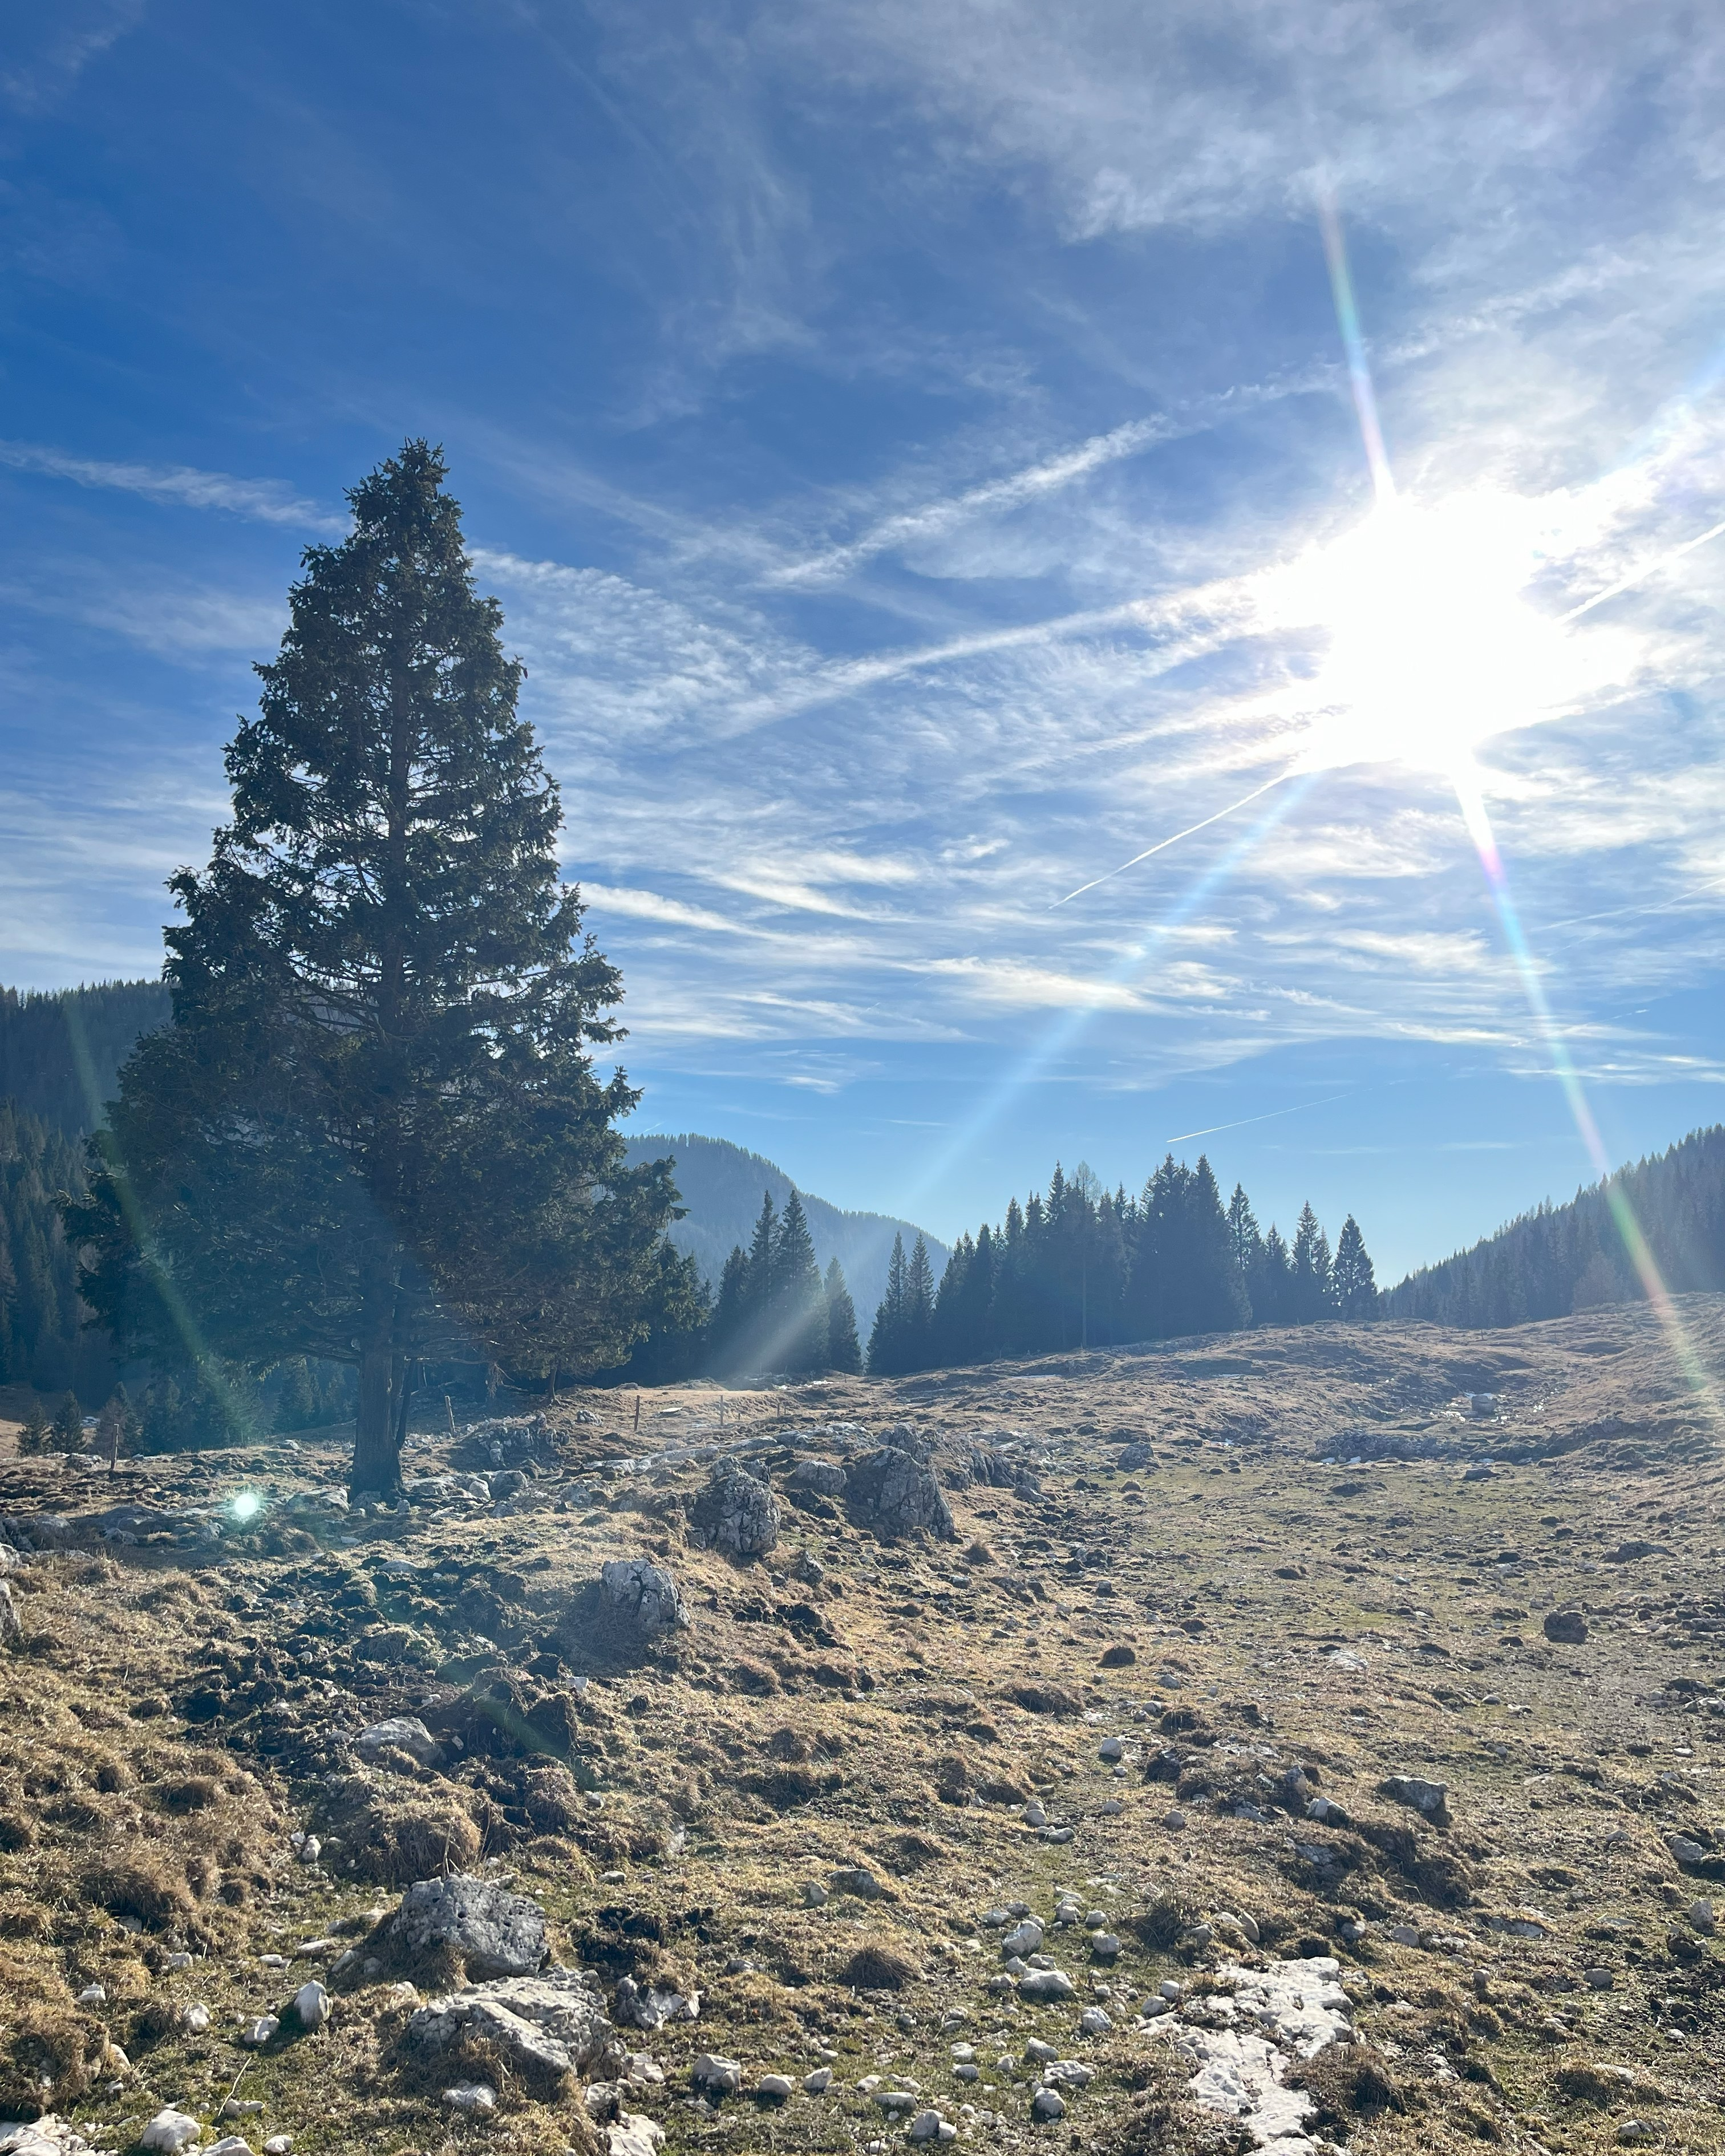
\includegraphics[width=\textwidth]{images/foto_paesaggio.jpg}
        \caption{Vista dal bivacco.}
        \label{fig:seconda_foto}
    \end{subfigure}

    \vspace{1em} % Aggiunge un po' di spazio tra la riga sopra e la foto sotto
    % Terza immagine sotto
    \begin{subfigure}[b]{\textwidth}
        \includegraphics[width=\textwidth]{images/foto_panoramica.jpg}
        \caption{Panoramica.}
        \label{fig:terza_foto}
    \end{subfigure}
    \caption{Selezione di fotografie del percorso e della vista dal bivacco.}
    \label{fig:foto}
\end{figure}

\end{document}
